\section{Экспериментальная проверка применимости метода на суперкомпьютере}
	Применимость метода оценивалась с помощью запусков приложений на суперкомпьютере "<Ломоносов-2">. Вычислительные узлы которого включают процессор Intel Haswell-EP E5-2697v3 (2.6 GHz), оборудованы 64 GB памяти и связаны коммуникационной сетью InfiniBand FDR \cite{Lom2_stat}.

	В качестве приложений для тестирования использовались реализации HPL, HPCG, алгоритмов DNS и SUMMA матричного умножения, Graph500. Так как рассматривается слабая масштабируемость, то тестирования проводились с конфигурациями запуска, удовлетворяющими выражению \eqref{weak_sc}. Для того чтобы более полно проверить применимость метода на реальных суперкомпьютерных приложениях и оценить их возможности к слабой масштабируемости, для некоторых из приложений тестирования проводились для нескольких значений констант используемых в этом выражении (HPL - 3 различных константы; Graph500, DNS - 2 различных константы; HPCG, SUMMA - 1 константа).

	Используемые обозначения в таблицах и рисунках:
	\begin{itemize}
		\item PN - количество процессов, на которых производится запуск задачи
		\item PS - размер задачи
		\item SC - scalefactor
		\item EF - edgefactor
		\item RE\_time - относительная ошибка предсказания времени
		\item RE\_perf - относительная ошибка предсказания производительности
	\end{itemize}
	Размер задачи во всех таблицах и рисунках измеряется в тысячах единиц, кроме HPCG и Graph500.

	\subsection{HPL}
	HPL (High Performance Computing Linpack Benchmark) — тест производительности вычислительной системы, на основе результатов которого формируется современный список TOP500 \cite{top500} лучших суперкомпьютеров в мире. Суть теста заключается в решении плотных систем линейных алгебраических уравнений, используя LU факторизацию, на системах с распределённой памятью.

	HPL имеет сложность алгоритма \(\mathcal{O}(N^3)\), а количество операций чтения/записи пропорционально \(\mathcal{O}(N^2)\). То есть, если размер задачи увеличить в два раза, то количество операций с плавающей запятой увеличится в восемь раз, в то время, как количество операций с памятью увеличится только в четыре раза. Подобные значения асимптотик свойственны приложениям с большим количеством вычислений над плотными структурами данных, такие приложения часто используют в своей работе графические ускорители.

	\begin{table}
		\centering
		\begin{tabular}{|r||c|c||c|c||c|c|}
			\hline
			            & \multicolumn{2}{c|}{\(C_1\)} & \multicolumn{2}{c|}{\(C_2\)} & \multicolumn{2}{c|}{\(C_3\)} \\ \hline
			\textnumero &  PN &                     PS &  PN &                     PS &  PN & PS                     \\ \hline
			1           &   6 &                     18 &   4 &                     20 &   4 & 25                     \\ \hline
			2           &   8 &                     20 &   6 &                     23 &   9 & 33                     \\ \hline
			3           &  12 &                     23 &   8 &                   25,3 &  12 & 36,4                   \\ \hline
			4           &  16 &                     25 &  10 &                  27,35 &  16 & 40 					 \\ \hline
			5           &  20 &                     27 &  12 &                   28,9 &  25 & 46,4 					 \\ \hline
			6           &  27 &                     30 &  15 &                   31,1 &  35 & 52 					 \\ \hline
			7           &  40 &                     34 &  20 &                  34,35 &  42 & 55,2 					 \\ \hline
			8           &  42 &                     35 &  25 &                  36,82 &  49 & 58,1                   \\ \hline
			9           &  50 &                     37 &  30 &                   39,1 &  56 & 60,7                   \\ \hline
			10          &  60 &                     39 &  36 &                   41,6 &  64 & 63,5                   \\ \hline
			11          &  64 &                     40 &  49 &                   46,1 &  81 & 68,7                   \\ \hline
			12          &  80 &                     43 &  64 &                   50,4 & 110 & 76,1                   \\ \hline
			13          &  90 &                     45 &  70 &                  51,95 & 121 & 78,5                   \\ \hline
			14          &  98 &                     46 &  80 &                   54,3 & 144 & 83,2                   \\ \hline
			15          & 110 &                     48 &  81 &                   54,5 & 169 & 87,8                   \\ \hline
			16          & 125 &                     50 & 121 &                   62,3 & 182 & 90                     \\ \hline
			17          & 140 &                     52 & 144 &                  66,05 & 196 & 92,2                   \\ \hline
			18          & 156 &                  53,85 & 169 &                   69,6 & 210 & 94,4                   \\ \hline
		\end{tabular}
		\caption{Тестовые конфигурации запусков HPL для трёх различных значений констант}
		\label{test_HPL}
	\end{table}
	% \begin{table}
	% 	\begin{tabular}{|r||c|c|c|c||c|c|c|c||c|c|c|c|}
	% 		\hline
	% 		& \multicolumn{4}{|c|}{\(C_1\)} & \multicolumn{4}{|c|}{\(C_2\)} & \multicolumn{4}{|c|}{\(C_3\)} \\ \hline
	% 		\textnumero & PN & PS & RE\_time & RE\_perf & PN & PS & RE\_time & RE\_perf & PN & PS & RE\_time & RE\_perf \\ \hline
	% 		1 & 225 & 60,8 & 7,58 &	6,82 & 225 & 76,65 & 3,82 & 0,82 & 225 & 100,8 & 5,79 & 5,69 \\ \hline
	% 		2 & 400 & 73,7 & 1,79 & 1,90 & 400 & 92,85 & 7,53 & 16,35 & 400 & 117 & 7,73 & 7,73 \\ \hline
	% 		3 & 576 & 83,2 & 0,37 & 0,45 & 576 & 104,8 & 0,62 & 9,25 & 576 & 132 & 6,06 & 5,72 \\ \hline
	% 		4 & 784 & 92,2 & 0,12 & 0,09 & 784 & 116,1 & 1,42 & 10,59 & 784 & 146,3 & 7,42 & 6,95 \\ \hline
	% 		5 & 1369 & 111 & 0,16 & 0,07 & 1369 & 140 & 11,35 & 4,41 & 1369 & 176,2 & 0,02 & 1,69 \\ \hline
	% 	\end{tabular}
	% 	\caption{Целевые конфигурации запусков HPL для трёх различных значений констант и значения относительных ошибок предсказания времени и производительности на этих конфигурациях}
	% 	\label{target_HPL}
	% \end{table}
	\begin{table}
		\centering
		\begin{tabular}{|r||c|c|c|c|}
			\hline
			            & \multicolumn{4}{|c|}{\(C_1\)}     \\ \hline
			\textnumero &   PN &   PS & RE\_time & RE\_perf \\ \hline
			          1 &  225 & 60,8 &     7,58 & 6,82     \\ \hline
			          2 &  400 & 73,7 &     1,79 & 1,90     \\ \hline
			          3 &  576 & 83,2 &     0,37 & 0,45     \\ \hline
			          4 &  784 & 92,2 &     0,12 & 0,09     \\ \hline
			          5 & 1369 &  111 &     0,16 & 0,07     \\ \hline
			\hline
			            & \multicolumn{4}{|c|}{\(C_2\)}      \\ \hline
			\textnumero &   PN &    PS & RE\_time & RE\_perf \\ \hline
			          1 &  225 & 76,65 &     3,82 & 0,82     \\ \hline
			          2 &  400 & 92,85 &     7,53 & 16,35    \\ \hline
			          3 &  576 & 104,8 &     0,62 & 9,25     \\ \hline
			          4 &  784 & 116,1 &     1,42 & 10,59    \\ \hline
			          5 & 1369 &   140 &    11,35 & 4,41     \\ \hline
			\hline
			            & \multicolumn{4}{|c|}{\(C_3\)}      \\ \hline
			\textnumero &   PN &    PS & RE\_time & RE\_perf \\ \hline
			          1 &  225 & 100,8 &     5,79 & 5,69     \\ \hline
			          2 &  400 &   117 &     7,73 & 7,73     \\ \hline
			          3 &  576 &   132 &     6,06 & 5,72     \\ \hline
			          4 &  784 & 146,3 &     7,42 & 6,95     \\ \hline
			          5 & 1369 & 176,2 &     0,02 & 1,69     \\ \hline
		\end{tabular}
		\caption{Целевые конфигурации запусков HPL для трёх различных значений констант и значения относительных ошибок предсказания времени и производительности на этих конфигурациях}
		\label{target_HPL}
	\end{table}

	\begin{figure}
		\centering
		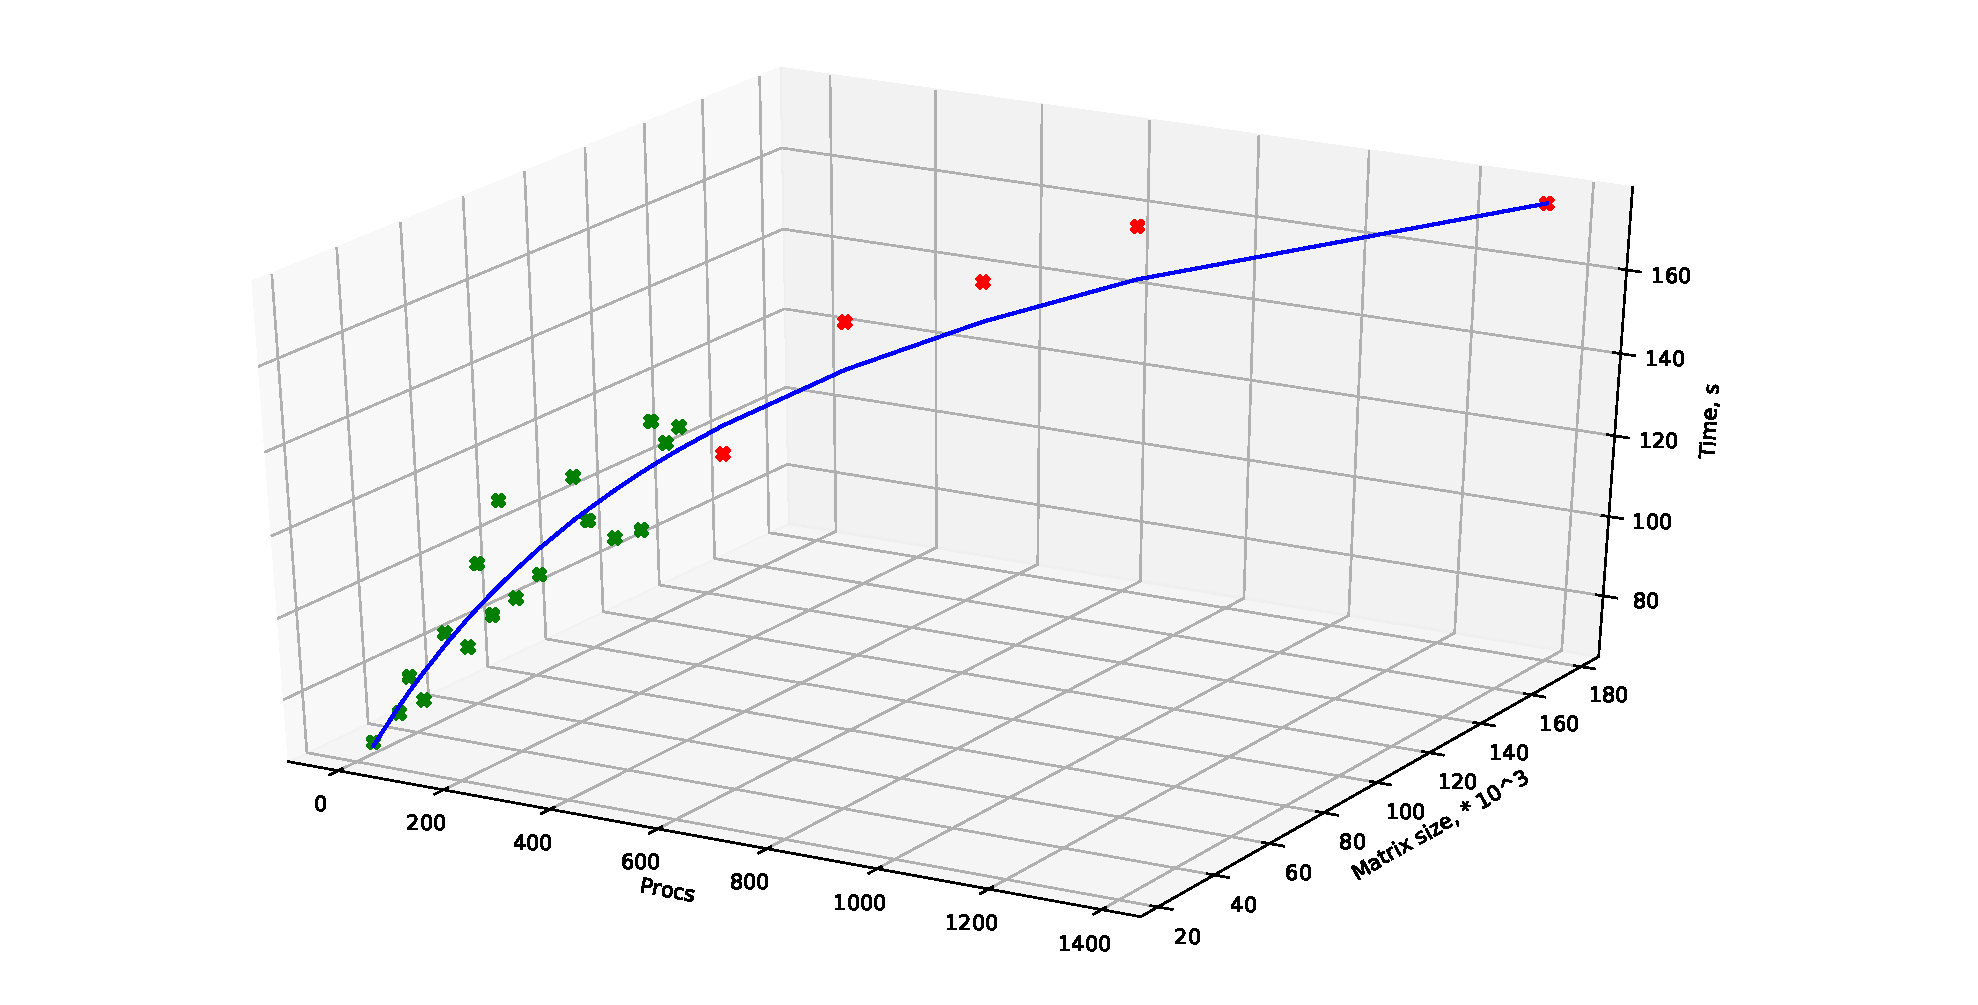
\includegraphics[width=0.9\textwidth]{./images/hpl_k3}
		\caption{Аппроксимирующая функция для слабой масштабируемости HPL, конфигурации соответствуют константе \(C_3\)}
		\label{figure_HPL_C_3}
	\end{figure}

	Тестовые конфигурации запуска, используемые для вычислений параметров модели, и целевых конфигураций, необходимые для оценки погрешности предсказаний, приведены в таблицах \eqref{test_HPL} и \eqref{target_HPL} соответственно. Коэффициенты \(C_1, C_2, C_3\), определяющие значение отношения количества работы приходящееся на один процесс и количества используемых процессов, из выражения \eqref{weak_sc}, связаны соотношением: \(4 \cdot C_1 = 2 \cdot C_2 = C_3 \), то есть с увеличением на единицу номера коэффициента количество работы на один процесс увеличивается в два раза.

	Относительные ошибки для всех целевых конфигураций слабой масштабируемости HPL представлены в таблице \eqref{target_HPL}. Значения относительных ошибок предсказания времени по всем целевым конфигурациям варьируются от 0,02\% до 11,35\%, среднее значение - 4,12\%, медиана - 3,82\%, а производительности - от 0,07\% до 16,35\%, среднее значение - 5,23\%, медиана - 5,69\%. Если рассматривать более детально, как меняются относительные ошибки с увеличением числа используемых процессов и размера задачи, усредняя значение ошибок по конфигурациям с одинаковым количеством используемых процессов, 225 - 5,09\%, 400 - 7,17\%, 576 - 3,74\%, 784 - 4,43\%, 1369 - 2,95\%, то можно однозначно сказать, что увеличение конфигурации не приводит к росту значений относительных ошибок. Что говорит об отсутствии необходимости увеличивать количество тестовых конфигураций и способности предложенного метода предсказывать значения различных динамических характеристик на конфигурациях в 6-7 раз больших, чем самые большие тестовые. Получающуюся аппроксимирующую функцию для одной из констант можно видеть на рисунке \eqref{figure_HPL_C_3}.

	\subsection{HPCG}

	HPCG (High Performance Conjugate Gradients Benchmark) был разработан, чтобы стать альтернативной HPL метрикой оценки производительности суперкомпьютеров. HPCG сильно выделяется на фоне остальных приложений, так как и сложность последовательного алгоритма, и количество операций чтения/записи бенчмарка пропорциональны \(\mathcal{O}(N)\). В тесте преобладают нерегулярный доступ к памяти и мелкоструктурные рекурсивные вычисления, которые свойственны многих научным вычислительным приложениям \cite{HPCG}. Основное вычислительное ядро HPCG занимается решением СЛАУ с разреженной положительно определённой симметричной матрицей с помощью метода сопряжённых градиентов.

	%Для тестирования использовались следующие конфигурации запуска: тестовые - количество процессов \(q = 14 \cdot i,\ i \in \{1 \ldots 15\}\), целевые - количество процессов \(q = 14 \cdot i,\ i \in \{20, 40, 50, 70, 100\}\), размер задачи для обоих случаев задаётся как - \(q \cdot 104 \cdot 104 \cdot 104\), то есть один процесс будет обсчитывать куб со стороной \(104\).
	Тестовые и целевые конфигурации представлены в таблице \eqref{conf_HPCG}, а получившиеся относительные ошибки предсказаний в таблице \eqref{result_HPCG}. Несмотря на то что в двух случая значения относительных ошибок сильно отличаются от остальных и почти достигают 20\%, среднее имеет гораздо более меньшее значения и составляет 2,674\% для предсказания времени и 8,554\% для производительности.
	\begin{table}
		\centering
		\begin{tabular}{|c|c|c|}
			\hline
			PN                          & PS                                 & Parameter \(i\)                                 \\ \hline
			\multirow{2}{*}{\(14 * i\)} & \multirow{2}{*}{\(104^3 * 14 *i\)} & Тестовые: \(i \in \{1,\,\ldots,\,15\}\)         \\ \cline{3-3}
			                            &                                    & Целевые:  \(i \in \{20,\,40,\,50,\,70,\,100\}\) \\ \hline
		\end{tabular}
		\caption{Тестовые и целевые конфигурации запусков HPCG}
		\label{conf_HPCG}
	\end{table}
	\begin{table}
		\centering
		\begin{tabular}{|c|c|c|}
			\hline
			PN   & RE\_time & RE\_perf \\ \hline
			280	 & 0,02     & 0,37     \\ \hline
			560	 & 1,56     & 0,80     \\ \hline
			700	 & 1,89     & 13,07    \\ \hline
			980	 & 2,85     & 19,54    \\ \hline
			1400 & 7,05     & 8,99     \\ \hline
		\end{tabular}
		\caption{Относительные ошибки предсказания времени и производительности HPCG}
		\label{result_HPCG}
	\end{table}

	\subsection{Алгоритмы матричного умножения}
		\subsubsection{SUMMA}
			Первый из двух рассматриваемых алгоритмов матричного умножения - SUMMA(Scalable Universal Matrix Multiply)\cite{SUMMA}. Этот алгоритм используется такими библиотеками, как ScaLAPACK и PBLAS. Он, так же как и HPL, имеет сложность \(\mathcal{O}(N^3)\) и количество операций чтения/записи пропорционально \(\mathcal{O}(N^2)\). Тестовые и целевые конфигурации запуска приведены в таблицах \eqref{test_SUMMA} и \eqref{target_SUMMA} соответственно. Для тестирования использовалась реализация, требующая квадратной процессорной сетки, однако в общем случае это не является обязательным условием для данного алгоритма. Коротко этот алгоритм можно записать так:
			\begin{algorithm}
				\begin{algorithmic}
					\State $C_{ij} = 0$
					\For{$l = \overline{0,k - 1}$}
					\State broadcast $a_i^l$ within my row
					\State broadcast $b_l^j$ within my column
					\State $C_{ij} = C_{ij} + a_i^l \cdot {b_l^j}^T$
					\EndFor
				\label{SUMMA_algo}
				\end{algorithmic}
			\end{algorithm}

			\begin{table}
				\centering
				\begin{tabular}{|r|c|c|}
					\hline
					            & \multicolumn{2}{c|}{\(C_1\)} \\ \hline
					\textnumero & PN  & PS                     \\ \hline
					1           & 1   & 4                      \\ \hline
					2           & 4   & 6,4                    \\ \hline
					3           & 9   & 8,4                    \\ \hline
					4           & 16  & 10                     \\ \hline
					5           & 25  & 11,5                   \\ \hline
					6           & 36  & 13,2                   \\ \hline
					7           & 49  & 14,7                   \\ \hline
					8           & 64  & 16                     \\ \hline
					9           & 81  & 17,1                   \\ \hline
					10          & 100 & 18,5                   \\ \hline
					11          & 121 & 19,8                   \\ \hline
					12          & 144 & 21                     \\ \hline
					13          & 169 & 22,1                   \\ \hline
					14          & 196 & 23,1                   \\ \hline
				\end{tabular}
				\caption{Тестовые конфигурации запусков матричного умножения по алгоритму SUMMA}
				\label{test_SUMMA}
			\end{table}

		\begin{table}
			\centering
			\begin{tabular}{|r|c|c|c|}
			\hline
			            & \multicolumn{3}{|c|}{\(C_1\)} \\ \hline
			\textnumero & PN   & PS   & RE\_time        \\ \hline
			1           & 225  & 25,6 & 1,95            \\ \hline
			2           & 400  & 30   & 3,94            \\ \hline
			3           & 576  & 33,6 & 3,01            \\ \hline
			4           & 784  & 37,8 & 7,59            \\ \hline
			5           & 1024 & 40   & 1,39            \\ \hline
			\end{tabular}
			\caption{Целевые конфигурации запусков матричного умножения по алгоритму SUMMA и значения относительных ошибок предсказания времени на этих конфигурациях}
			\label{target_SUMMA}
		\end{table}
		%Из-за того что исследуется предсказание масштабируемости в условиях слабой масштабируемости приложений, 
		Из-за того что строятся предсказания слабой масштабируемости приложений, то рассматриваемые конфигурации должны удовлетворят выражению \eqref{weak_sc} для некоторого значения константы. Так как известно, что данный алгоритм имеет кубическую сложность, то можно уточнить запись этого выражения: \(T_A(N)\:/\:p = const \Rightarrow p = N^3\:/\:const\). Как видно по графику зависимости количества используемых процессов от длины стороны матрицы \eqref{conf_SUMMA} конфигурации запусков выбираются строго согласно этому выражению.

		\begin{figure}
			\centering
			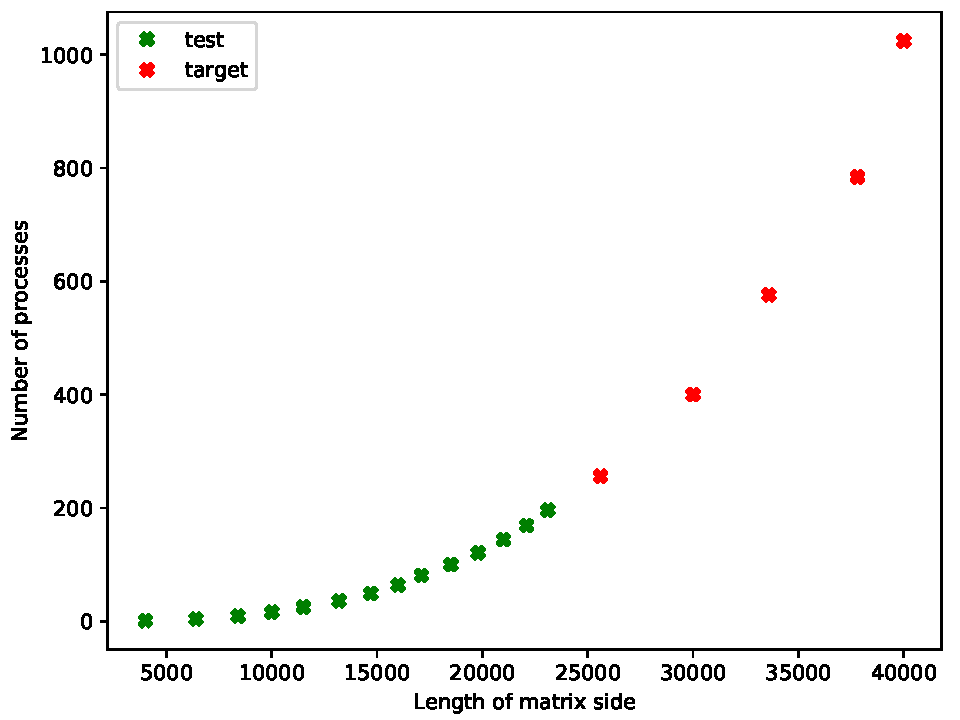
\includegraphics[width=0.5\textwidth]{./images/conf_SUMMA}
			\caption{Конфигурации запусков матричного умножения по алгоритму SUMMA}
			\label{conf_SUMMA}
		\end{figure}

		Не смотря на сложную, скачкообразную зависимость времени работы программы \eqref{graph_SUMMA} предложенному методу удаётся установить основной характер изменения и построить предсказание так, что среднее значение относительной ошибки равно 3,58\%, а медиана - 3,01\%, все значения относительных ошибок приведены в таблице \eqref{target_SUMMA}.

		\begin{figure}
			\centering
			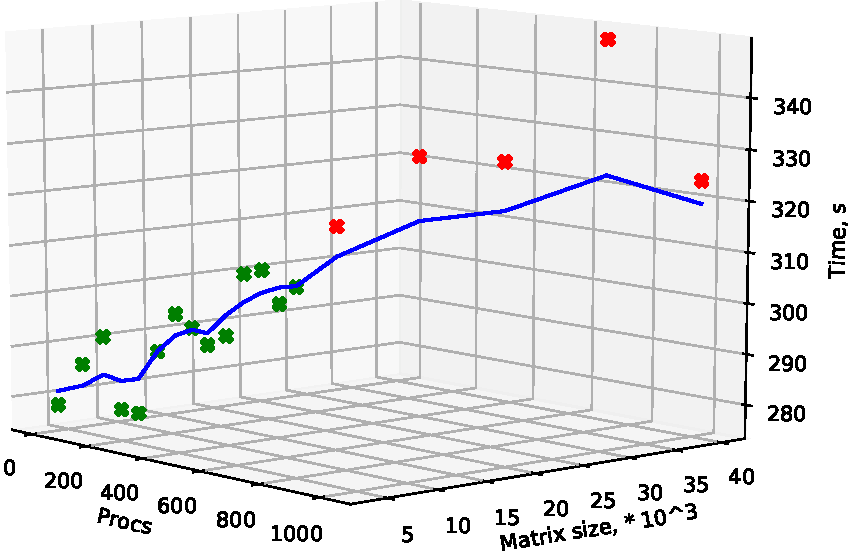
\includegraphics[width=0.9\textwidth]{./images/graph_SUMMA}
			\caption{Аппроксимирующая функция для слабой масштабируемости матричного умножения по алгоритму SUMMA}
			\label{graph_SUMMA}
		\end{figure}

		\subsubsection{DNS}
			Следующий из рассматриваемых алгоритмов матричного умножения - DNS. Для его работы необходимо, чтобы количество процессов было равно кубу некоторого натурального числа. Из этих процессов создаётся 3D решётка. Перемножаемые матрицы считываются нижним слоем решётки, делятся на блоки и рассылаются специальным образом остальным процессам. Далее происходит локальное перемножение полученных блоков матриц и пересылка получившихся значений на нижний слой, из которых там собирается результирующая матрица.

			\begin{table}
				\centering
				\begin{tabular}{|r||c|c||c|c|}
					\hline
					            & \multicolumn{2}{c||}{\(C_1\)} & \multicolumn{2}{c|}{\(C_2\)}  \\ \hline
					\textnumero & PN  & PS                      & PN  & PS                      \\ \hline
					1           & 1   & 4,5                     & 1   & 9                       \\ \hline
					2           & 8   & 9                       & 8   & 18                      \\ \hline
					3           & 27  & 13,5                    & 27  & 27                      \\ \hline
					4           & 64  & 18                      & 64  & 36                      \\ \hline
					5           & 125 & 22,5                    & 125 & 45                      \\ \hline
					6           & 216 & 27                      & 216 & 54                      \\ \hline
				\end{tabular}
				\caption{Тестовые конфигурации запусков матричного умножения по алгоритму DNS для двух различных значений констант}
				\label{test_DNS}
			\end{table}

			\begin{table}
				\centering
				\begin{tabular}{|r||c|c|c||c|c|c|}
					\hline
					            & \multicolumn{3}{|c||}{\(C_1\)} & \multicolumn{3}{c|}{\(C_2\)} \\ \hline
					\textnumero & PN   & PS   & RE\_time        & PN   & PS & RE\_time          \\ \hline
					1           & 343  & 31,5 & 6,55            & 343  & 63 & 5,66              \\ \hline
					2           & 512  & 36   & 8,42            & 512  & 72 & 6,84              \\ \hline
					3           & 729  & 40,5 & 9,35            & 729  & 81 & 7,85              \\ \hline
					4           & 1000 & 45   & 7,94            & 1000 & 90 & 1,94              \\ \hline
					5           & 1331 & 49,5 & 9,63            & 1331 & 99 & 0,19              \\ \hline
				\end{tabular}
				\caption{Целевые конфигурации запусков DNS для двух различных значений констант и значения относительных ошибок предсказания времени и производительности на этих конфигурациях}
				\label{target_DNS}
			\end{table}

			Из-за ограничения, накладываемого алгоритмом на количество используемых для запуска процессов, тестовая выборка получается достаточно маленькая, всего 6 различных конфигураций. Но, несмотря на это, среднее значение относительной ошибки составляет всего 6,43\%. Получившиеся функции-предикторы для двух рассматриваемых значений констант представлены на рисунках \eqref{graph_DNS}. С некоторого момента при увеличением размера конфигурации, независимо от рассматриваемой константы, время работы алгоритма почти прекращает расти, это говорит об его хорошей слабой масштабируемости, а то небольшое увеличение времени работы можно связать с возрастающими накладными расходами на коммуникации.

			\begin{figure}
			\begin{subfigure}{.5\textwidth}
				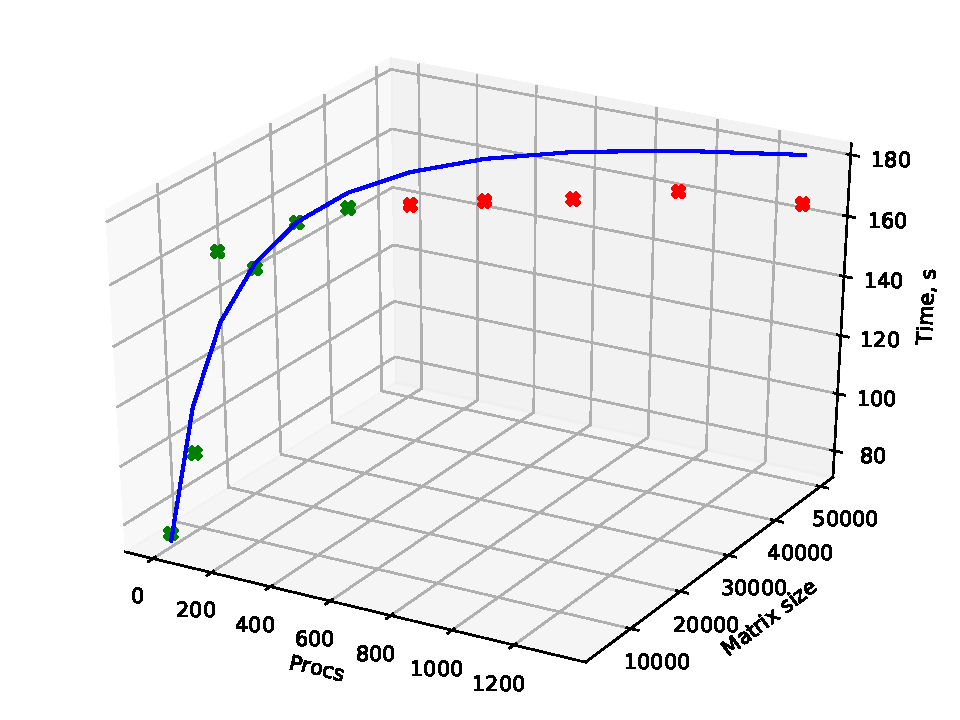
\includegraphics[width=\linewidth]{./images/graph_C_1_DNS}
				\caption{\(C_1\)}
				\label{graph_C_1_DNS}
			\end{subfigure}
			\begin{subfigure}{.5\textwidth}
				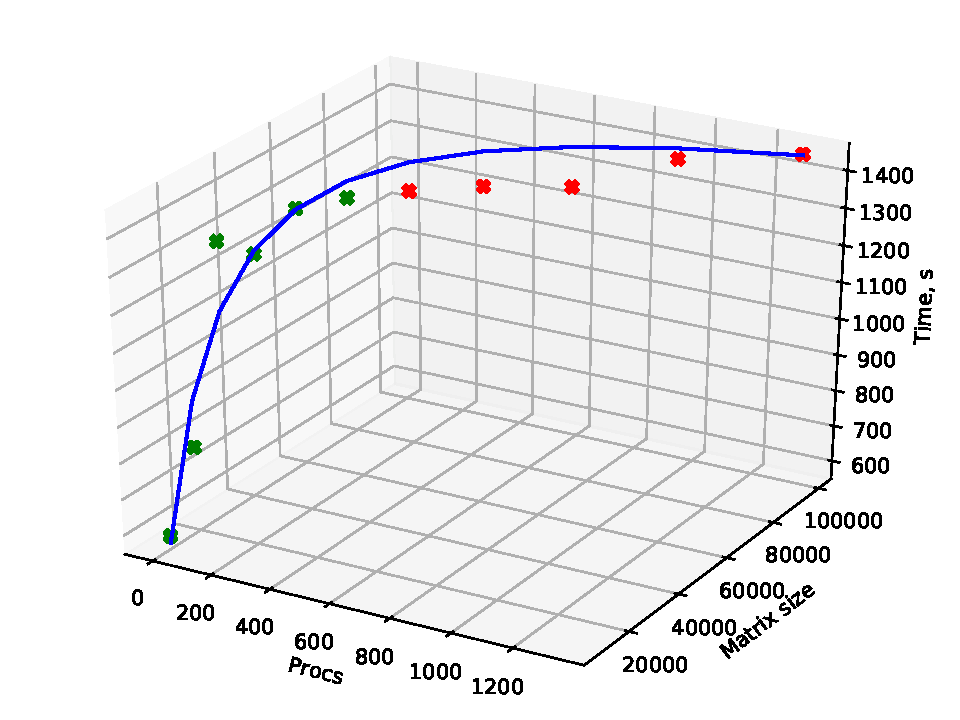
\includegraphics[width=\linewidth]{./images/graph_C_2_DNS}
				\caption{\(C_2\)}
				\label{graph_C_2_DNS}
			\end{subfigure}
			\caption{Аппроксимирующие функции предсказания времени выполнения матричного умножения по алгоритму DNS для двух различных значений констант}
			\label{graph_DNS}
			\end{figure}

	\subsection{Graph500}
		Последнее из рассматриваемых приложений - Graph500. Это ещё одна альтернатива HPL, помимо уже ранее рассмотренного бенчмарка HPCG, по результатам работы которого также составляется рейтинг суперкомпьютеров. Однако Graph500, в отличии от HPL и HPCG, больше нагружает коммуникационную подсистему компьютера и не так сильно зависит от количества исполняемых операций над числами с плавающей запятой в секунду. Подобное поведение свойственно многим задачам из области графовой аналитики и работы с большими данными. Бенчмарк Graph500 включает в себя два графовых алгоритма: поиск в ширину (BFS) и поиск кратчайшего пути от одной вершины (SSSP). Из-за того, что в основе лежит работа с графами, то производительность измеряется не в GFlops, а в MTeps (количество пройденных дуг в секунду).

		Сложность алгоритма в случае работы с графами выражается через число его вершин и рёбер, так для Graph500 это \(\mathcal{O}(V + E)\), где \(V\)- количество вершин, а \(E\) - рёбер. Размер задачи задаётся двумя параметрами \(scale - SC\) и \(edgefactor - EF\): количество вершин графа равно \(2^{SC}\), а \(EF\) равен половине средней степени вершины графа, то есть \(EF = \frac{E}{V}\). Используя эти два параметра для вычисления сложности работы алгоритма, можно получить: \[V + E = 2^{SC} + EF \cdot 2^{SC} = 2^{SC} \cdot (1 + EF) \]

		\begin{table}
			\centering
			\begin{tabular}{|r||c|c|c||c|c|c|}
				\hline
				            & \multicolumn{3}{c||}{\(C_1\)} & \multicolumn{3}{c|}{\(C_2\)} \\ \hline
				\textnumero & PN  & SC & EF                 & PN  & SC & EF                \\ \hline
				1           & 14  & 25 & 16                 & 14  & 26 & 16                \\ \hline
				2           & 28  & 26 & 16                 & 28  & 27 & 16                \\ \hline
				3           & 42  & 26 & 25                 & 42  & 27 & 25                \\ \hline
				4           & 56  & 27 & 16                 & 56  & 28 & 16                \\ \hline
				5           & 70  & 27 & 20                 & 70  & 28 & 20                \\ \hline
				6           & 84  & 27 & 25                 & 84  & 28 & 25                \\ \hline
				7           & 98  & 27 & 29                 & 98  & 28 & 29                \\ \hline
				8           & 112 & 28 & 16                 & 112 & 29 & 16                \\ \hline
				9           & 126 & 28 & 18                 & 126 & 29 & 18                \\ \hline
				10          & 140 & 28 & 20                 & 140 & 29 & 20                \\ \hline
				11          & 154 & 28 & 22                 & 154 & 29 & 22                \\ \hline
				12          & 168 & 28 & 25                 & 168 & 29 & 25                \\ \hline
				13          & 182 & 28 & 27                 & 182 & 29 & 27                \\ \hline
				14          & 196 & 29 & 14                 & 196 & 30 & 14                \\ \hline
				15          & 210 & 29 & 15                 & 210 & 30 & 15                \\ \hline
			\end{tabular}
			\caption{Тестовые конфигурации запусков бенчмарка Graph500 для двух различных значений констант}
			\label{test_Graph500}
		\end{table}

		\begin{table}
			\centering
			\begin{tabular}{|r||c|c|c|c|c|c|c|}
				\hline
				            & \multicolumn{7}{c|}{\(C_1\)}                                                     \\ \hline
				            & PN   & SC & EF & RE\_time(BFS) & RE\_perf(BFS) & RE\_time(SSSP) & RE\_perf(SSSP) \\ \hline
				1           & 280  & 30 & 20 &          3,23 &          4,20 &           6,40 & 7,06           \\ \hline
				2           & 560  & 31 & 20 &          5,09 &          2,03 &          17,62 & 17,67          \\ \hline
				3           & 700  & 31 & 26 &         12,94 &          8,82 &           5,24 & 9,99           \\ \hline
				4           & 980  & 31 & 36 &         20,93 &         19,92 &           0,61 & 5,76           \\ \hline
				5           & 1400 & 32 & 26 &         15,59 &          8,54 &           5,29 & 12,98          \\ \hhline{|=||=|=|=|=|=|=|=|} 
				            & \multicolumn{7}{c|}{\(C_2\)}                                                     \\ \hline
				\textnumero & PN   & SC & EF & RE\_time(BFS) & RE\_perf(BFS) & RE\_time(SSSP) & RE\_perf(SSSP) \\ \hline
				1           & 280  & 29 & 20 &         12,42 &         12,03 &          16,87 & 15,05          \\ \hline
				2           & 560  & 30 & 20 &          5,08 &          7,86 &          25,16 & 21,94          \\ \hline  
				3           & 700  & 30 & 26 &          5,74 &          0,50 &          27,14 & 24,63          \\ \hline
				4           & 980  & 30 & 36 &         25,80 &         27,76 &           8,41 & 11,22          \\ \hline
				5           & 1400 & 31 & 26 &         26,45 &         24,55 &          19,61 & 21,93          \\ \hline

				              
			\end{tabular}
			\caption{Целевые конфигурации запусков бенчмарка Graph500 для двух различных значений констант и значения относительных ошибок предсказания времени и производительности на этих конфигурациях}
			\label{targer_Graph500}
		\end{table}

		Во время тестирования этого приложения становится ясно видна основная проблема определения, предсказывания слабой масштабируемости приложений: конфигурации запуска выбираются согласно отношению \eqref{weak_sc}, но не всегда возможно обеспечить строгое равенство, поэтому приходится округлять некоторые параметры запуска. Из-за этого возможны провалы или всплески показателей рассматриваемых динамических характеристик, которые сильно портят качество предсказаний. Так в случае Graph500 приходилось округлять значения \(SC\) и \(EF\), так как они могут принимать только целые значения. В связи с этим средние значения относительных ошибок предсказания времени и производительности для этого приложения составляют около 13\%.
\clearpage
%\newpage